\documentclass[12pt]{beamer}

\usetheme[progressbar=frametitle]{metropolis}

\usepackage{booktabs}
\usepackage[scale=2]{ccicons}

\usepackage{pgfplots}
\usepgfplotslibrary{dateplot}
\usepackage{texshade}      

\usepackage{xspace}
\usepackage{xcolor}
\usepackage{tikz}
\usepackage{forest}
\usetikzlibrary{arrows.meta}

\newcommand{\themename}{\textbf{\textsc{metropolis}}\xspace}
\newcommand{\red}[1]{\textcolor{red}{#1}}
\newcommand{\blue}[1]{\textcolor{blue}{#1}}
\newcommand{\green}[1]{\textcolor{green}{#1}}
\newcommand{\yellow}[1]{\textcolor{yellow}{#1}}

\setbeamercovered{invisible}

\title{Phylogenetic Footprinting Methods for determining TFBS}
\subtitle{}
\date{\today}
\author{Saket Choudhary}
%\institute{Center for modern beamer themes}
%\titlegraphic{\hfill\includegraphics[height=1.5cm]{logo}}

\begin{document}

\maketitle

\begin{frame}{Table of contents}
  \setbeamertemplate{section in toc}[sections numbered]
  \tableofcontents[hideallsubsections]
\end{frame}

\section{Introduction}
{
\setbeamertemplate{frame footer}{Wasserman, W. W., \& Sandelin, A. (2004)}
\begin{frame}[fragile]{TFs bind to specific sites on DNA}

\begin{figure}
\includegraphics[width=0.8\linewidth]{images/crm.jpg}
\end{figure}
 
\end{frame}
}

\begin{frame}[fragile]{Discovering TFBS: Properties}
  \begin{columns}[T,onlytextwidth]
    \column{0.5\textwidth}
\begin{itemize}
\item Short sequences (5-25bp)
\item Proximity to TSS (~100-1000bp)
\item Degeneracy
\end{itemize}
\column{0.5\textwidth}
\uncover<2->{\begin{texshade}{images/aln-msf.txt}
\setends{1}{1..5}
\hidenumbering
\showsequencelogo{top}
\showconsensus[ColdHot]{bottom}
\defconsensus{.}{lower}{upper}
\end{texshade}}
\end{columns}
\end{frame}


\begin{frame}[fragile]{Motif Representation}
  \begin{columns}[T,onlytextwidth]
    \column{0.5\textwidth}
\begin{itemize}[<+- | alert@+>]
\item Consensus: $max_\alpha(n_\alpha^{(i)})$
\item Frequency Matrix: $n_{\alpha}^{(i)}/N$
\item PWM: $\log_2\frac{f_\alpha^{(i)}}{p_{\alpha}}$
\item Information: $2+\sum_\alpha \log_2\frac{f_\alpha^{(i)}}{p_{\alpha}}$
\end{itemize}
\column{0.5\textwidth}

\uncover<1->{\begin{texshade}{images/aln-msf.txt}
\setends{1}{1..5}
\hidenumbering
\showsequencelogo{top}
\showconsensus[ColdHot]{bottom}
\defconsensus{.}{lower}{upper}
\end{texshade}}

\end{columns}
\end{frame}

\begin{frame}[fragile]{Discovering TFBS: Analogous to Clustering}
`Discovery' is different from `finding':
\begin{itemize}
\item Discovery involves identifying meaningful patterns :: Identifying clusters
\item `Identifying' involves speicific positions given the pattern :: Assigning datapoints to clusters
\end{itemize}
\end{frame}

\begin{frame}[fragile]{Motif Discovery Approaches}
Two axes of information
\begin{itemize}[<+- | alert@+>]
\item Over-representation
\item Cross-specie conservation
\end{itemize}
\end{frame}

\begin{frame}[fragile]{Over-representation}

\begin{figure}
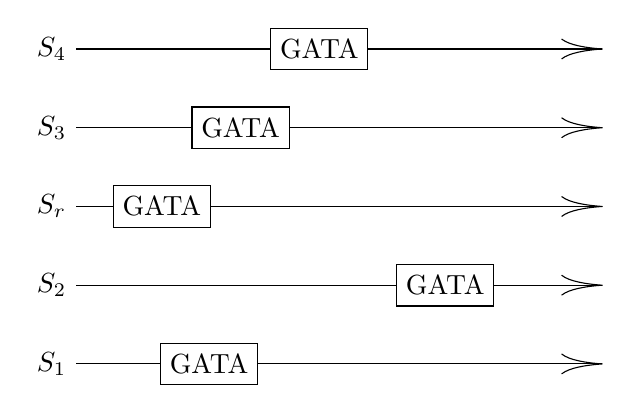
\begin{tikzpicture}
    \tikzstyle{operator} = [draw,fill=white,minimum size=1.5em] 
    \node at (0,0) (q1) {$S_1$};
    \node at (0,1) (q2) {$S_2$};
    \node at (0,2) (qr) {$S_r$};
    \node at (0,3) (q3) {$S_3$};
    \node at (0,4) (q4) {$S_4$};
        
    \node[operator] (op11) at (2,0) {GATA} edge [-] (q1);
    \draw[-{>[scale=2.5,
          length=6,
          width=3]}](op11) -- (7,0);

    \node[operator] (op21) at (5,1) {GATA} edge [-] (q2);
    \draw[-{>[scale=2.5,
          length=6,
          width=3]}] (op21) -- (7,1);

    \node[operator] (opr1) at (1.4,2) {GATA} edge [-] (qr);
    \draw[-{>[scale=2.5,
          length=6,
          width=3]}](opr1) -- (7,2);
    
    \node[operator] (op31) at (2.4,3) {GATA} edge [-] (q3);
    \draw[-{>[scale=2.5,
          length=6,
          width=3]}] (op31) -- (7,3);

    \node[operator] (op41) at (3.4,4) {GATA} edge [-] (q4);
    \draw[-{>[scale=2.5,
          length=6,
          width=3]}] (op41) -- (7,4);

    
\end{tikzpicture}
\end{figure}
\end{frame}


\begin{frame}[fragile]{Cross-Specie conservation}

\begin{figure}
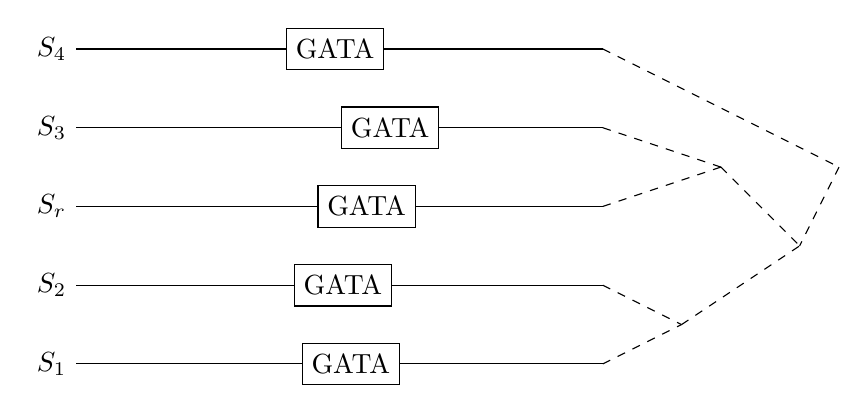
\begin{tikzpicture}
    \tikzstyle{operator} = [draw,fill=white,minimum size=1.5em] 
    \node at (0,0) (q1) {$S_1$};
    \node at (0,1) (q2) {$S_2$};
    \node at (0,2) (qr) {$S_r$};
    \node at (0,3) (q3) {$S_3$};
    \node at (0,4) (q4) {$S_4$};
        
    \node[operator] (op11) at (3.8,0) {GATA} edge [-] (q1);
    \draw(op11) -- (7,0);
    \draw[dashed](7,0) -- (8,0.5);
    \draw[dashed](8,0.5) -- (9.5, 1.5);

    \node[operator] (op21) at (3.7,1) {GATA} edge [-] (q2);
    \draw (op21) -- (7,1);
    \draw[dashed](7,1) -- (8,0.5);

    \node[operator] (opr1) at (4,2) {GATA} edge [-] (qr);
    \draw(opr1) -- (7,2);
    \draw[dashed](7,2) -- (8.5,2.5);
    
    \node[operator] (op31) at (4.3,3) {GATA} edge [-] (q3);
    \draw(op31) -- (7,3);
    \draw[dashed](7,3) -- (8.5,2.5);
    \draw[dashed](8.5,2.5) -- (9.5, 1.5);

    \node[operator] (op41) at (3.6,4) {GATA} edge [-] (q4);
    \draw(op41) -- (7,4);
    \draw[dashed](7,4) -- (10, 2.5);
	\draw[dashed](10,2.5) -- (9.5,1.5);    
    
\end{tikzpicture}
\end{figure}
\end{frame}


\begin{frame}{References}
  Some references to showcase [allowframebreaks] \cite{knuth92,ConcreteMath,Simpson,Er01,greenwade93}
\end{frame}

\section{Conclusion}

\begin{frame}{Summary}


\end{frame}

\begin{frame}[standout]
  Thank You!
\end{frame}

\appendix

\begin{frame}[fragile]{Backup slides}
  Sometimes, it is useful to add slides at the end of your presentation to
  refer to during audience questions.

  The best way to do this is to include the \verb|appendixnumberbeamer|
  package in your preamble and call \verb|\appendix| before your backup slides.

  \themename will automatically turn off slide numbering and progress bars for
  slides in the appendix.
\end{frame}

\begin{frame}[allowframebreaks]{References}

  \bibliography{demo}
  \bibliographystyle{abbrv}

\end{frame}

\end{document}
